\documentclass[a4paper,12pt]{report}
\usepackage[utf8]{inputenc}
\usepackage{amsmath} % For mathematical symbols and environments
\usepackage{graphicx} % For including graphics
\usepackage{geometry} % For adjusting page margins
\usepackage{listings}
\usepackage{xcolor}
\usepackage{enumitem} % For customizing lists
\usepackage{float}


% Define the style for C code
\lstset{
    language=C,
    basicstyle=\ttfamily\small,  % Set the basic font style
    keywordstyle=\color{blue},   % Color of keywords
    commentstyle=\color{green},  % Color of comments
    stringstyle=\color{red},     % Color of strings
    numberstyle=\tiny\color{gray}, % Line numbers
    frame=single,                % Frame around the code
    breaklines=true,             % Break long lines
}

\renewcommand{\thesection}{\arabic{section}}
% Set custom margins
\geometry{
  top=1in,    % Top margin
  bottom=1in, % Bottom margin
  left=1in, % Left margin
  right=1in % Right margin
}
% Define custom title format with subtitle and roll number
\title{
  \vspace{-2em} % Adjust the space above the title
  \textbf{CS-700 Algorithms and Complexity} \\ % Main title
  \large \textbf{Assignment-1} \\ % Subtitle
  \vspace{1em} % Space between subtitle and author
  \textbf{ANAND M K} \\ % Author
  Roll Number: 242CS008 \\% Roll number
  Department of Computer Science and Engg.- NITK Surathkal
}

\date{} % Remove the date

\begin{document}

\maketitle

\section{Introduction}
In this assignment, I have analyzed and compared different sorting algorithms based on their execution time. The performance of these algorithms was compared with varying input sizes, and an in-depth analysis has been conducted.

The following sorting algorithms were considered for comparison:
\begin{itemize}
  \item Bubble Sort
  \item Insertion Sort
  \item Merge Sort
  \item Quick Sort
  \item Heap Sort
  \item Radix Sort
\end{itemize}

\section{Data Generation and Experimental Setup}
\subsection{Input Data}
Three different versions of input data were considered for each algorithm:
\begin{enumerate}
  \item Elements sorted in increasing order.
  \item Elements sorted in decreasing order.
  \item Randomly generated elements.
\end{enumerate}

The program can read the input from a file and execute the code. The format of the input files is as follows:
\begin{verbatim}
[n] //number of positive integers to sort
[element 1]
[element 2]
...
...
[element n]
\end{verbatim}

Where \( n \) varies from 10,000 to 100,000, with intervals of 10,000. For each version of input data, there are 10 input files, each corresponding to a different input data size ranging from 10,000 to 100,000. This varied dataset allows for a more comprehensive analysis.

\newpage
\subsection{Machine Specifications}
\begin{itemize}
  \item CPU: 11th Gen Intel® Core™ i5-11500 @ 2.70GHz × 12
  \item RAM: 16 GiB
  \item Operating System: Ubuntu 22.04.4 LTS
  \item Compiler: gcc 11.4.0
\end{itemize}

\subsection{Timing Mechanism}
Execution time was calculated in milliseconds using the gettimeofday() function in C, which provides higher precision than the clock() function. The <sys/time.h> header file is required for gettimeofday(). The following code was used to calculate the execution time.
\begin{lstlisting}
    struct timeval start, end;
    gettimeofday(&start, NULL);
    Sorting Algorithm();
    gettimeofday(&end, NULL);
    double executiontime = (end.tv_sec - start.tv_sec) + ((end.tv_usec - start.tv_usec) / 1000000.0); // Execution time in seconds
    executiontime = executiontime * 1000; // Execution time in milli seconds
\end{lstlisting}

\subsection{Experiment Repetitions}
Each experiment was repeated more than 10 times to verify that the measurements were valid and did not produce incorrect values.

\subsection{Time Capture}
Each sorting algorithm was executed with different input sizes, and the time was captured for each case. The time was calculated as the average of multiple repetitions of the experiments. 

\subsection{Input Generation and Selection}
I have generated the input files as follows:

\begin{itemize}[label=--]
    \item \textbf{For the increasing order file:} Numbers were generated from 100,000 to 100,000 plus the size of the input file.\\
    \textit{Example:} For an increasing order file with 20,000 numbers, the values will range from 100,000 to 120,000.
    
    \item \textbf{For the decreasing order file:} Numbers were generated from 200,000 to 200,000 minus the size of the input file.\\
    \textit{Example:} For a decreasing order file with 20,000 numbers, the values will range from 200,000 to 180,000.
    
    \item \textbf{For the file with random values:} Numbers were generated using the \texttt{rand()} function in C, with values between 100,000 and 200,000.
\end{itemize}

\subsection{Input Consistency: Were the same inputs used for all sorting algorithms?}
Yes, the same set of inputs was used for all sorting algorithms.

\section{Analysis of QuickSort}
Three versions of QuickSort have been considered for analysis:
\begin{itemize}
    \item \textbf{Version 1:} The first element in the array.
    \item \textbf{Version 2:} A random element in the array.
    \item \textbf{Version 3:} The median of the first, middle, and last elements in the array.
\end{itemize}

\subsection{Version 1 : QuickSort with the Pivot as the First Element} 

\begin{itemize}
    \item \textbf{Sorted List in Increasing Order:} Since the pivot is selected as the first element, each partitioning step is highly unbalanced. Therefore, the time complexity results in \(O(n^2)\).
    
    \item \textbf{Sorted List in Decreasing Order:} Similar to the increasing order list, the pivot choice leads to highly unbalanced partitions. Thus, the time complexity also results in \(O(n^2)\).
    
    \item \textbf{Random Order List:} In this case, the list is not sorted, so the pivot does not consistently produce unbalanced partitions. As a result, the algorithm performs better, and the time complexity is approximately \(O(n \log n)\).
\end{itemize}
\begin{figure}[H]
    \centering
    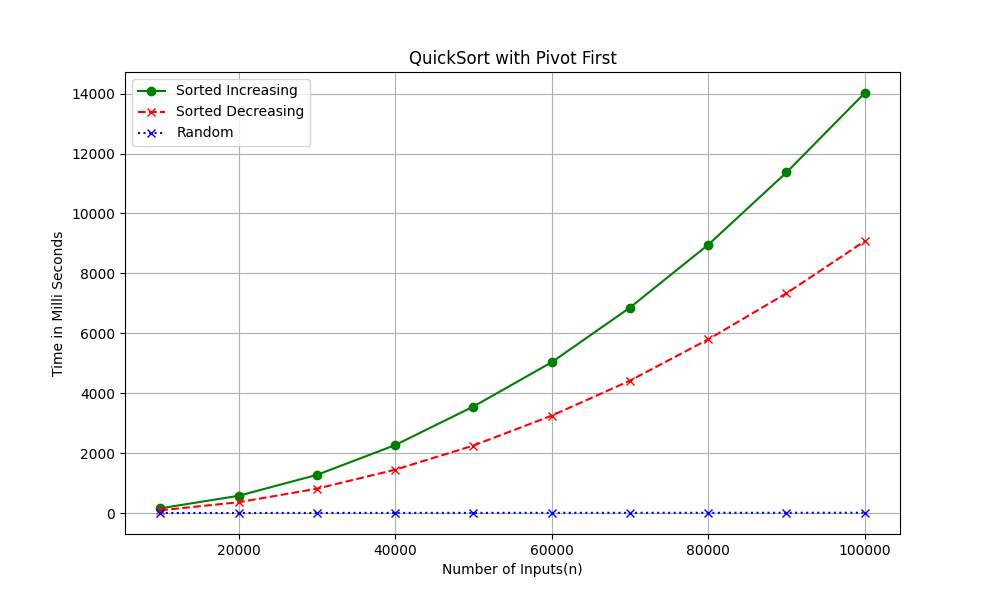
\includegraphics[width=1.1\textwidth]{./QuickSortPivotFirst.png}
    \caption{Performance of QuickSort with Pivot as the First Element}
    \label{fig:quicksort_performance}
\end{figure}

\subsection{Version 2 : QuickSort with the Pivot as the Random Element} 

\begin{itemize}
    \item \textbf{Sorted List in Increasing Order:} Since the pivot is chosen randomly, each partitioning step is less likely to be highly unbalanced. This results time complexity of \(O(n \log n)\). 
    
    \item \textbf{Sorted List in Decreasing Order:} Similar to the sorted increasing order list, the random pivot selection helps avoid consistently poor partitioning. Therefore, the time complexity is \(O(n \log n)\). 

    \item \textbf{Random Order List:} The random pivot selection generally provides balanced partitions and ensures good performance. The  time complexity is \(O(n \log n)\)
\end{itemize}
\begin{figure}[H]
    \centering
    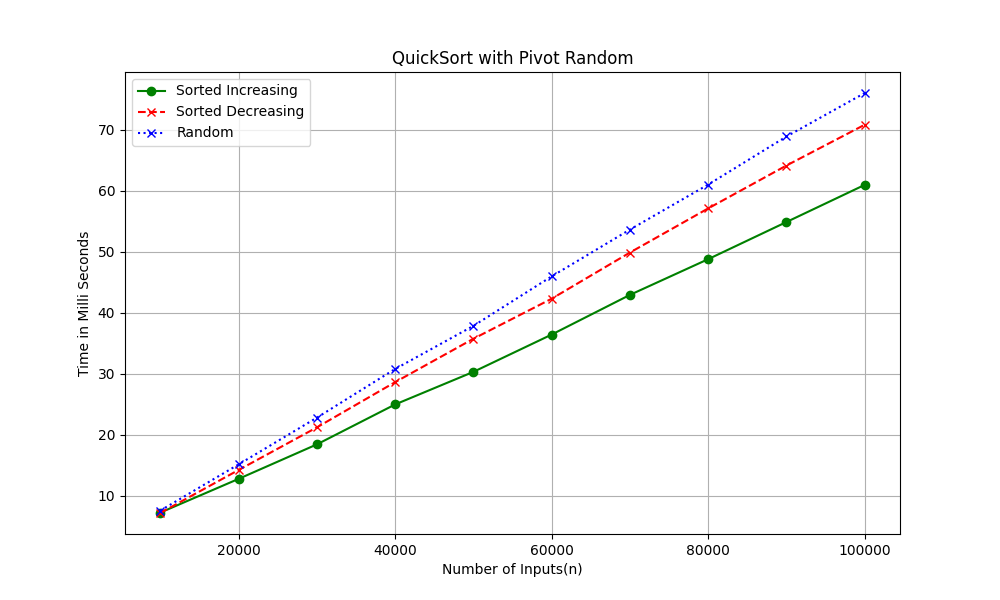
\includegraphics[width=1.1\textwidth]{./QuickSortPivotRandom.png}
    \caption{Performance of QuickSort with Random Pivot Choice}
    \label{fig:quicksort_random_pivot}
\end{figure}

\subsection{Version 3 : QuickSort with the Pivot as the Median of the First, Middle, and Last Elements} 
\begin{itemize}
    \item \textbf{Sorted List in Increasing Order:} The median of the first, middle, and last elements as the pivot generally results in more balanced partitions, as it chooses a pivot more likely to be near the middle value. This results in an average time complexity of \(O(n \log n)\). 

    \item \textbf{Sorted List in Decreasing Order:}  Similar to the increasing order list, the median as the pivot choice improves partitioning, and the time complexity results in \(O(n \log n)\).

    \item \textbf{Random Order List:} The median pivot selection generally provides balanced partitions and ensures good performance. The time complexity is \(O(n \log n)\).
\end{itemize}

\begin{figure}[H]
    \centering
    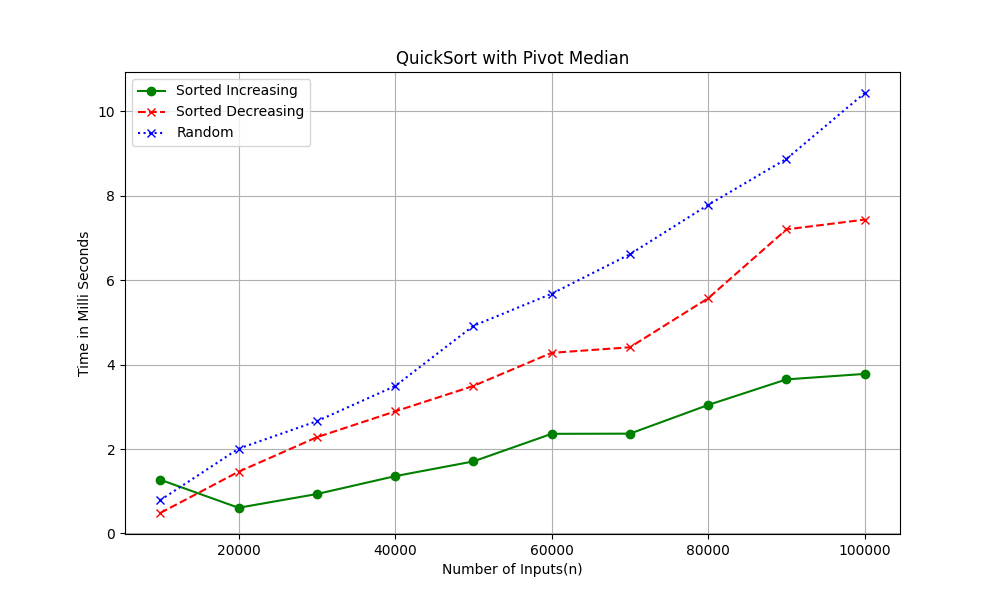
\includegraphics[width=1.1\textwidth]{./QuickSortPivotMedian.png}
    \caption{Performance of QuickSort with Pivot as the Median of the First, Middle, and Last Elements}
    \label{fig:quicksort_median_pivot}
\end{figure}

\subsection{Best Case Performance of Three Versions of Quick Sort}
As per the above analysis, the best case occurs when the partitions are balanced, and there are fewer unbalanced partitions. This leads to a best-case time complexity of \(O(n \log n)\) in all three versions.
\begin{itemize}
    \item \textbf{Version 1:} As per the above experiments and observations, the random array gives the best case.

    \item \textbf{Version 2:} Even though all types of inputs result in \(O(n \log n)\), considering the experiments conducted and the graph, the sorted array in increasing order gives the best times.

    \item \textbf{Version 3:} Even though all types of inputs result in \(O(n \log n)\), considering the experiments conducted and the graph, the sorted array in increasing order gives the best times.
\end{itemize}
Following Figure-4 shows the best case running time for all the three versions of quick
sort.
\begin{figure}[H]
    \centering
    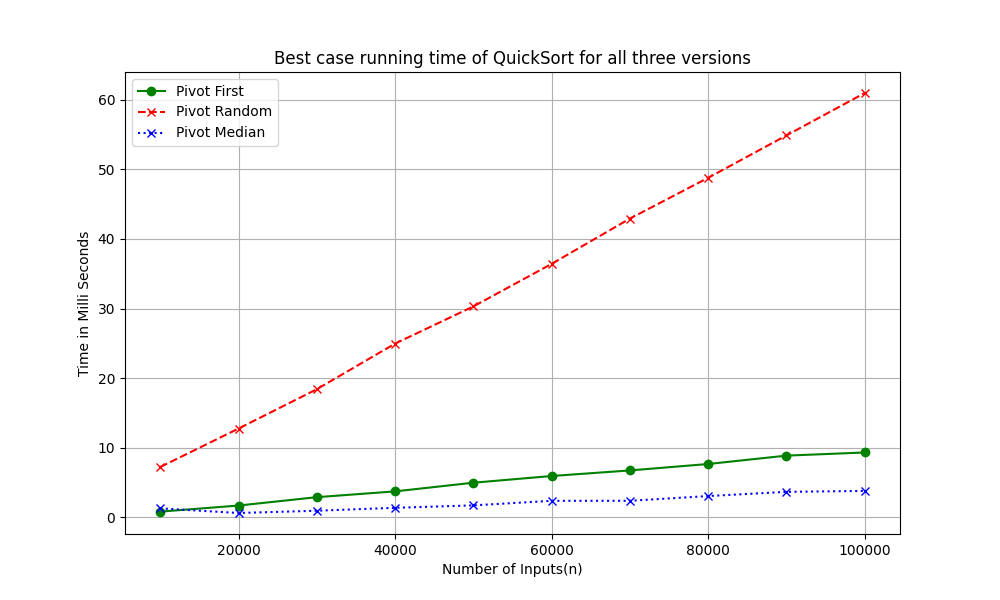
\includegraphics[width=1.1\textwidth]{./Best_case_QuickSort.png}
    \caption{Best case running time of QuickSort for all three versions}
    \label{fig:Best case of quicksort}
\end{figure}

\subsection{Worst Case Performance of Three Versions of Quick Sort}
Worst case occurs when partitions are highly unbalanced, which leads to a worst-case time complexity of \(O(n^2)\).
\begin{itemize}
    \item \textbf{Version 1:} For both sorted lists (increasing and decreasing), when the pivot is the first element, it leads to unbalanced partitions and a time complexity of \(O(n^2)\). Though both the increasing and decreasing arrays have the same time complexity of \(O(n^2)\), the experiments show that the increasing array results in the worst time.

    \item \textbf{Version 2:} When the pivot is selected randomly, there is a very low chance of getting an unbalanced partition. The worst case occurs when the randomly selected pivot consistently picks extreme values (either the smallest or largest element), which is highly unlikely. According to experiments and analysis, all three inputs result in the same time complexity of \(O(n \log n)\), but the random order array yields the worst time among them.

    \item \textbf{Version 3:} Similar to the case with a random pivot, using the median of the first, middle, and last elements as the pivot generally prevents the worst-case scenario. According to the experiments, while all input versions have a time complexity of \(O(n \log n)\), the random order array results in the worst performance.

\end{itemize}
Following Figure-5 and Figure-6 shows worst case running time of all the three versions of quick sort
\begin{figure}[H]
    \centering
    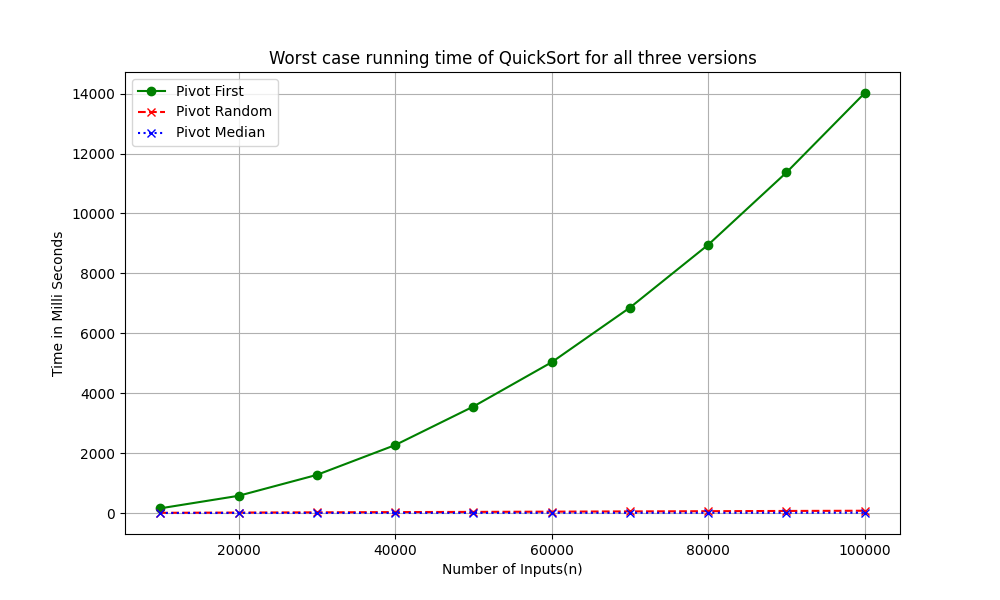
\includegraphics[width=1.1\textwidth]{./Worst_case_QuickSort.png}
    \caption{Worst case running time of QuickSort for all three versions}
    \label{fig:Worst case quicksort}
\end{figure}

\begin{figure}[H]
    \centering
    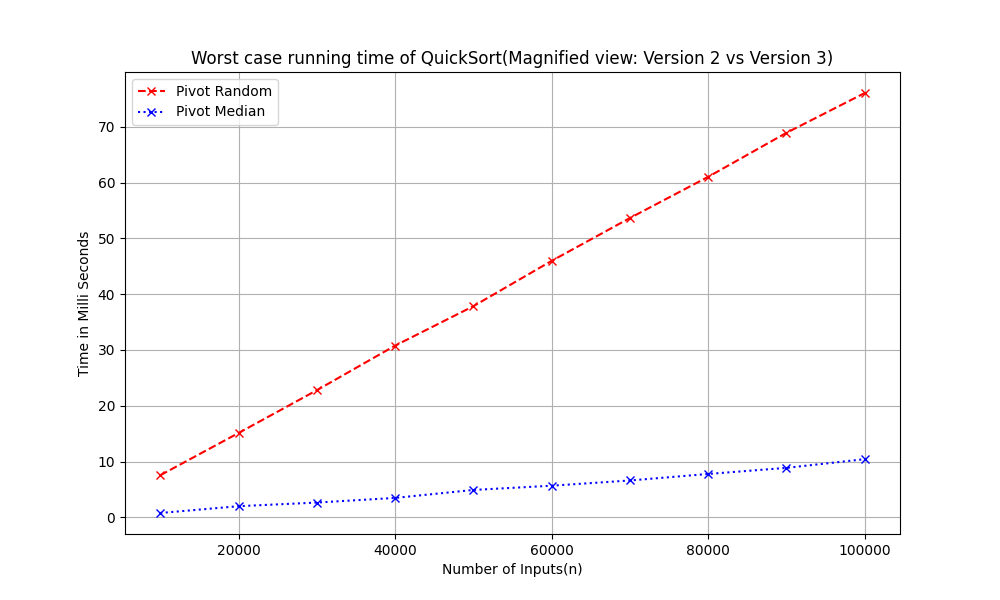
\includegraphics[width=1.1\textwidth]{./Worst_case_QuickSort _Magnified_view.png}
    \caption{Worst case running time of QuickSort(Magnified view: Version 2 vs Version 3)}
    \label{fig:Worst case quicksort Magnified}
\end{figure}

\subsection{Average Case Performance of Three Versions of Quick Sort}
All three versions of QuickSort yield an average time complexity of \(O(n \log n)\).
\begin{itemize}
	\item \textbf{Version 1:} When the array is neither fully sorted nor completely unbalanced, balanced partitions occur on average, leading to an average time complexity of \(O(n \log n)\). For analyzing the average case, a different input file was considered where parts of the array are sorted, and other parts are shuffled.
	
	\item \textbf{Version 2:} When the pivot is selected randomly, the average case also results in a time complexity of \(O(n \log n)\). The random pivot choice tends to create balanced partitions on average, leading to efficient sorting in most cases.
	
	\item \textbf{Version 3:} Using the median of the first, middle, and last elements as the pivot generally produces more balanced partitions, resulting in an average case time complexity of \(O(n \log n)\). This method minimizes the chances of extreme unbalanced partitions, ensuring consistent performance across different input types.
\end{itemize}
Following Figure-7 and Figure-8 shows Average case running time of all the three versions of quick sort
\begin{figure}[H]
	\centering
	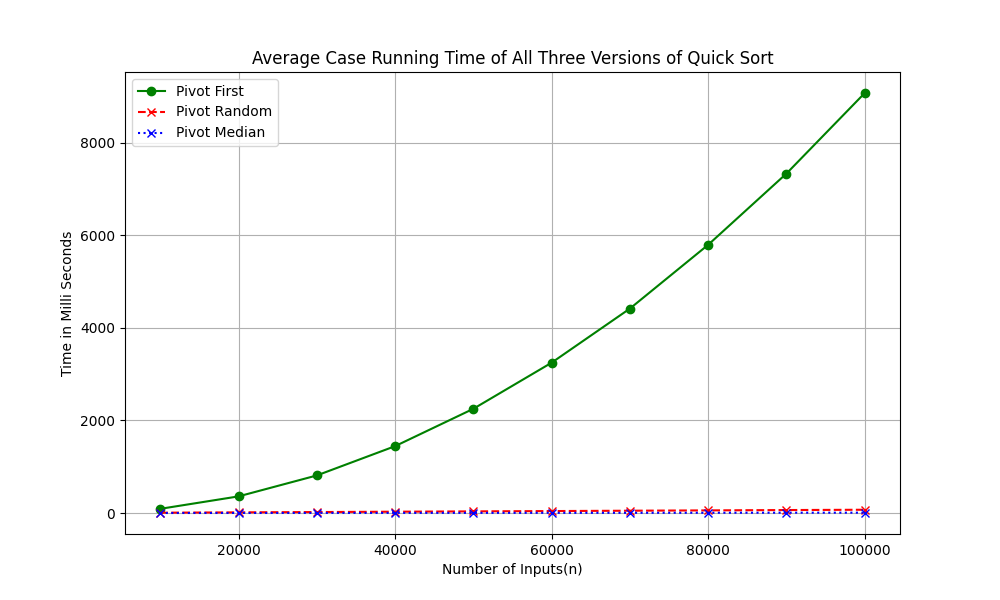
\includegraphics[width=1.1\textwidth]{./Average_case_QuickSort.png}
	\caption{Average case running time of QuickSort for all three versions}
	\label{fig:Average case quicksort}
\end{figure}

\begin{figure}[H]
	\centering
	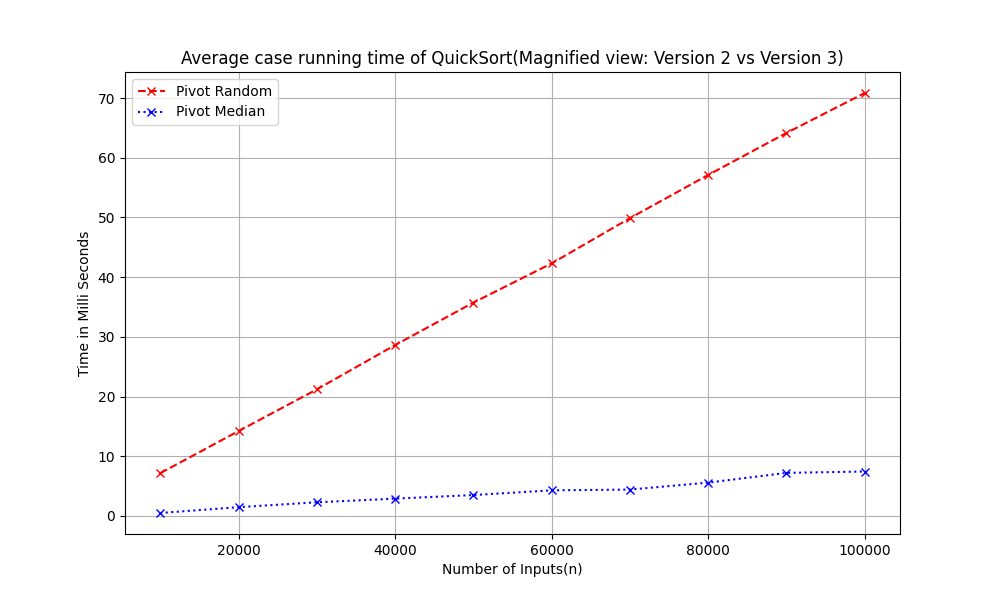
\includegraphics[width=1.1\textwidth]{./Average_case_QuickSort_Magnified_view.png}
	\caption{Average case running time of QuickSort(Magnified view: Version 2 vs Version 3)}
	\label{fig:Average case quicksort Magnified}
\end{figure}

\subsection{Conclusion of Quicksort Analysis}
By considering all the analyses, the median-based pivot is the most reliable, minimizing the chances of extremely unbalanced partitions and consistently providing a time complexity of O(n log n) across all three input versions. This is followed by the random pivot, with the first-element pivot being the least favorable.
 
\section{Analysis of All Six Sorting Algorithms}

\subsection{Analysis of Best Case}
The best case for each of the six algorithms is different and occurs on various inputs. The following best cases are based on practical experiments and the execution time collected from actual performance. The theoretical time complexity is also included.
\begin{itemize}
    \item \textbf{Bubble Sort:} According to practical observations, a sorted array in increasing order yields the best times. However, the differences in execution times across all three input types are minimal, indicating that the order of input has little impact on the time. Theoretically, the time complexity for all three input versions is \(O(n^2)\). The graph also reflects this with a line representing \(O(n^2)\). \emph{(Note: I have considered the standard Bubble Sort, not the optimized version.)}
    
    \item \textbf{Insertion Sort:} Practical observations show that a sorted array in increasing order produces the best times. Theoretically, the time complexity for the best case is \(O(n)\), and the graph represents this as well.
    
    \item \textbf{Merge Sort:} Practical observations indicate that the execution times for all three inputs are almost identical, with only minor differences. This suggests that the order of input has little impact on execution time. Theoretically, the time complexity for all three input versions is \(O(n \log n)\).
    
    \item \textbf{Quick Sort (Median Pivot):} Practical observations reveal that a sorted array in increasing order yields the best times. However, the differences in execution times across all three inputs are minimal, implying that the order of input has little effect on execution time. Theoretically, the time complexity for all three input versions is \(O(n \log n)\).
    
    \item \textbf{Heap Sort:} Practical observations show that a sorted array in decreasing order yields the best times, but the differences in execution times across all three inputs are minimal. This indicates that the order of input has little impact on execution time. Theoretically, the time complexity for all three input versions is \(O(n \log n)\).
    
    \item \textbf{Radix Sort:} Practical observations indicate that the execution times for all three inputs are nearly identical, with only slight differences, suggesting that the order of input has little impact on execution time. Theoretically, the time complexity for all three input versions is \(O(n)\).
\end{itemize}
Following Figure-9 and Figure-10 shows Best case running time of all the sorting algorithms. 
\begin{figure}[H]
	\centering
	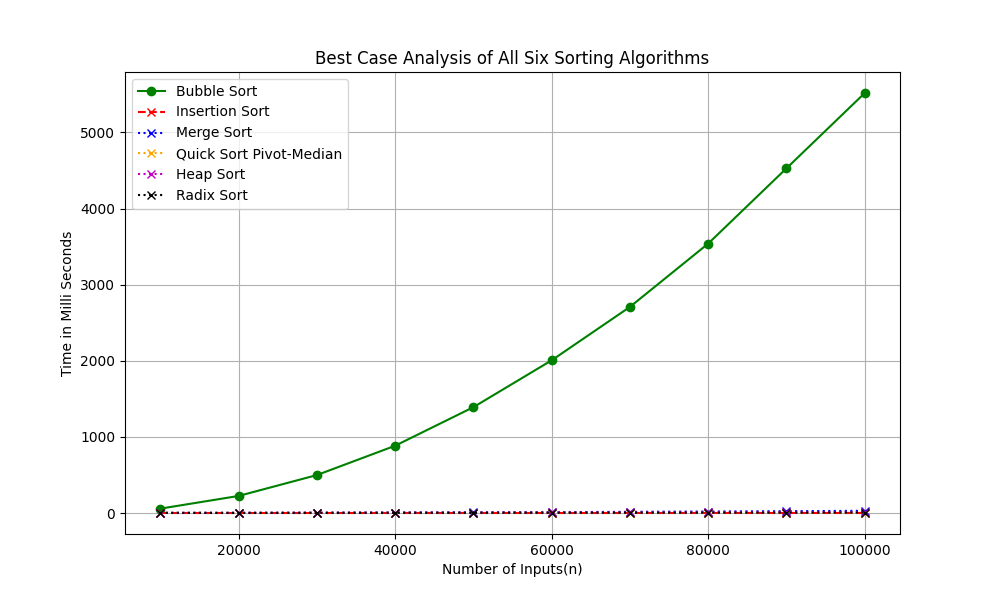
\includegraphics[width=1.1\textwidth]{./Bestofall.png}
	\caption{Best case running time of all the sorting algorithms}
	\label{fig:Best of all}
\end{figure}

\begin{figure}[H]
	\centering
	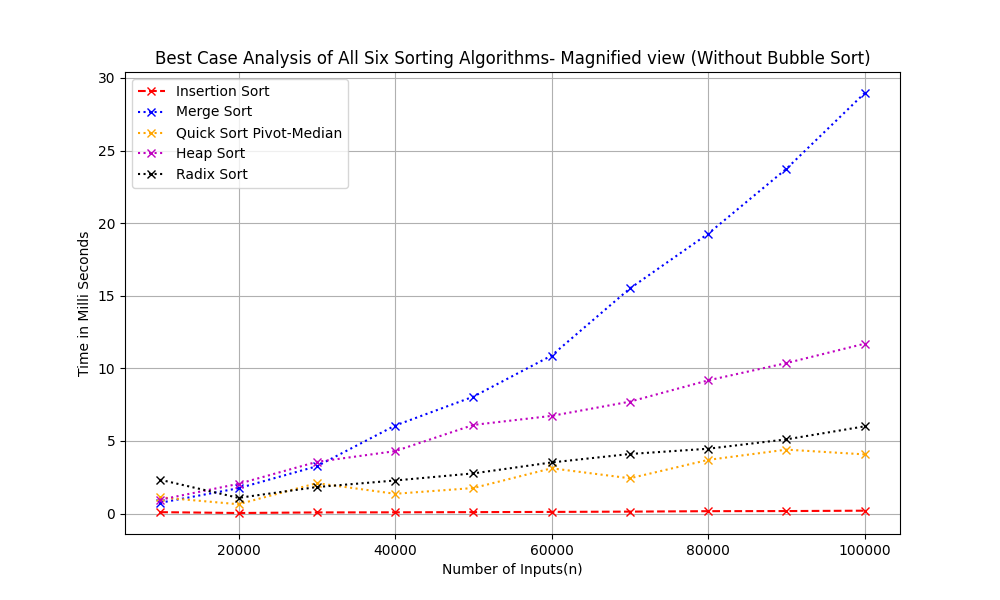
\includegraphics[width=1.1\textwidth]{./BestofallMagnified.png}
	\caption{Best case running time of all the sorting algorithms(Magnified view: Without Bubble Sort)}
	\label{fig:Best of all Magnified}
\end{figure}

\subsection{Analysis of Worst Case}
\begin{itemize}
    \item \textbf{Bubble Sort:} According to practical observations, the random array yields the worst execution time. However, the differences in execution times across all three input types are minimal, indicating that the order of input has little impact on the time. Theoretically, the time complexity for all three input versions is \(O(n^2)\). \emph{(Note: I have considered the standard Bubble Sort, not the optimized version.)}
    
    \item \textbf{Insertion Sort:} Practical observations show that, sorted array in decreasing order produces the worst times. Theoretically, the time complexity for the worst case is \( O(n^2) \).
    
    \item \textbf{Merge Sort:} Practical observations indicate that the execution times for all three inputs are almost identical, with only minor differences. This suggests that the order of input has little impact on execution time. Theoretically, the time complexity for all three input versions is \(O(n \log n)\).
    
    \item \textbf{Quick Sort (Median Pivot):} Practical observations reveal that, random array yields the worst performance times. However, the differences in execution times across all three inputs are minimal, implying that the order of input has little effect on execution time. Theoretically, the time complexity for all three input versions is \(O(n \log n)\).
    
    \item \textbf{Heap Sort:} Practical observations show that random array yields the worst execution times, but the differences in execution times across all three inputs are minimal. This indicates that the order of input has little impact on execution time. Theoretically, the time complexity for all three input versions is \(O(n \log n)\).
    
    \item \textbf{Radix Sort:} Practical observations indicate that the execution times for all three inputs are nearly identical, with only slight differences, suggesting that the order of input has little impact on execution time. Theoretically, the time complexity for all three input versions is \(O(n)\).
\end{itemize}
Following Figure-11 and Figure-12 shows Worst case running time of all the sorting algorithms. 
\begin{figure}[H]
	\centering
	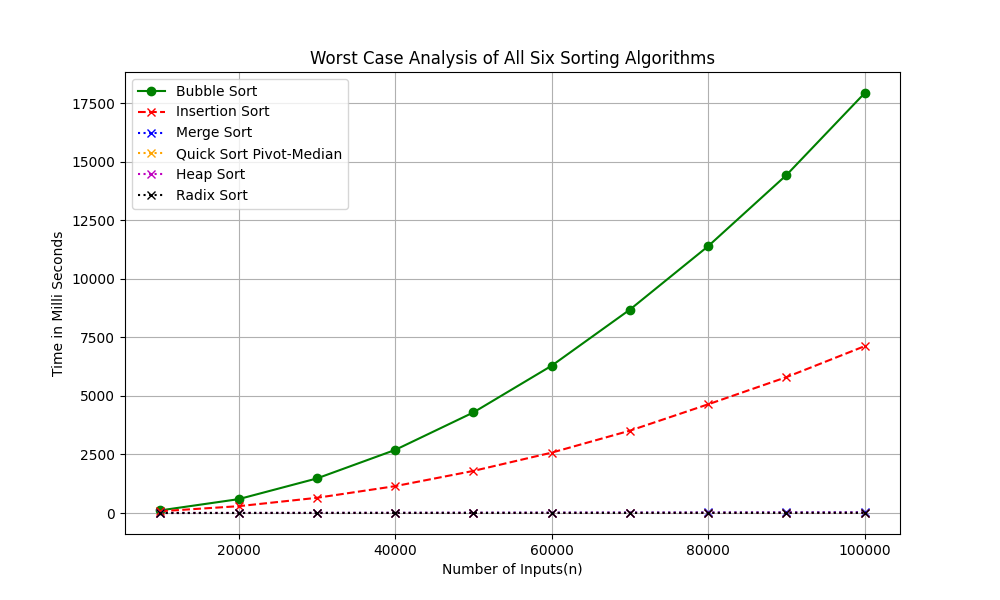
\includegraphics[width=1.1\textwidth]{./Worstofall.png}
	\caption{Worst case running time of all the sorting algorithms}
	\label{fig:Worst of all}
\end{figure}

\begin{figure}[H]
	\centering
	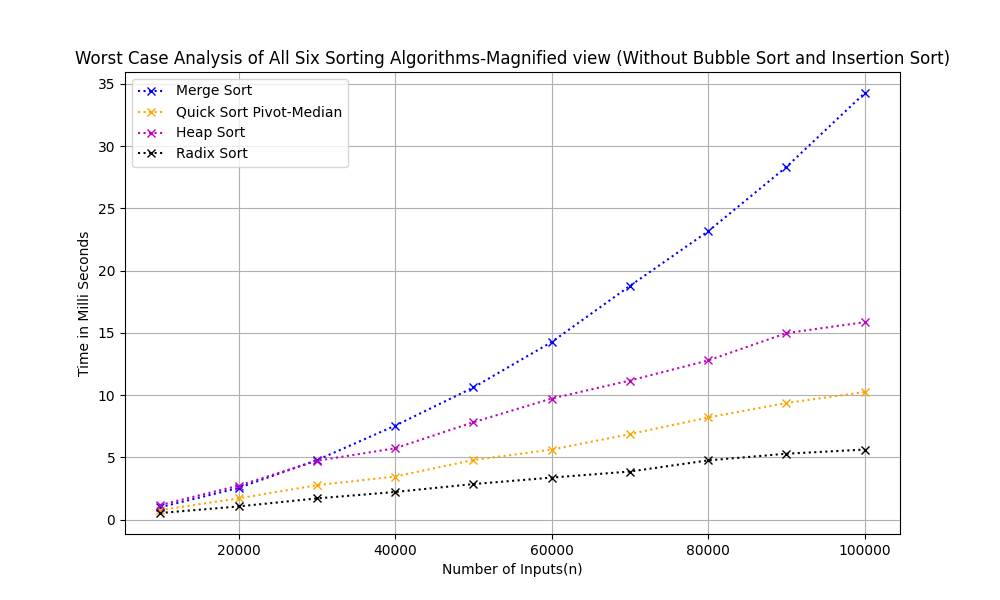
\includegraphics[width=1.1\textwidth]{./Worstofallmagnified.png}
	\caption{Worst case running time of all the sorting algorithms(Magnified view: Without Bubble Sort and Insertion Sort)}
	\label{fig:Worst of all Magnified}
\end{figure}

\subsection{Analysis of Average Case}
\begin{itemize}
    \item \textbf{Bubble Sort:} According to practical observations, sorted array in decreasing order yields average execution times. However, the differences in execution times across all three input types are minimal, indicating that the order of input has little impact on the time. Theoretically, the time complexity for all three input versions is \(O(n^2)\). \emph{(Note: I have considered the standard Bubble Sort, not the optimized version.)}
    
    \item \textbf{Insertion Sort:} Practical observations show that a random array has average execution times. Theoretically, the time complexity for the average case is \( O(n^2) \).
    
    \item \textbf{Merge Sort:} Practical observations indicate that the execution times for all three inputs are almost identical, with only minor differences. This suggests that the order of input has little impact on execution time. Theoretically, the time complexity for all three input versions is \(O(n \log n)\).
    
    \item \textbf{Quick Sort (Median Pivot):} Practical observations reveal that sorted array in decreasing order yields average execution times. However, the differences in execution times across all three inputs are minimal, implying that the order of input has little effect on execution time. Theoretically, the time complexity for all three input versions is \(O(n \log n)\).
    
    \item \textbf{Heap Sort:} Practical observations show that sorted array in increasing order yields average execution times, but the differences in execution times across all three inputs are minimal. This indicates that the order of input has little impact on execution time. Theoretically, the time complexity for all three input versions is \(O(n \log n)\).
    
    \item \textbf{Radix Sort:} Practical observations indicate that the execution times for all three inputs are nearly identical, with only slight differences, suggesting that the order of input has little impact on execution time. Theoretically, the time complexity for all three input versions is \(O(n)\).
\end{itemize}
Following Figure-13 and Figure-14 shows Average case running time of all the sorting algorithms. 
\begin{figure}[H]
	\centering
	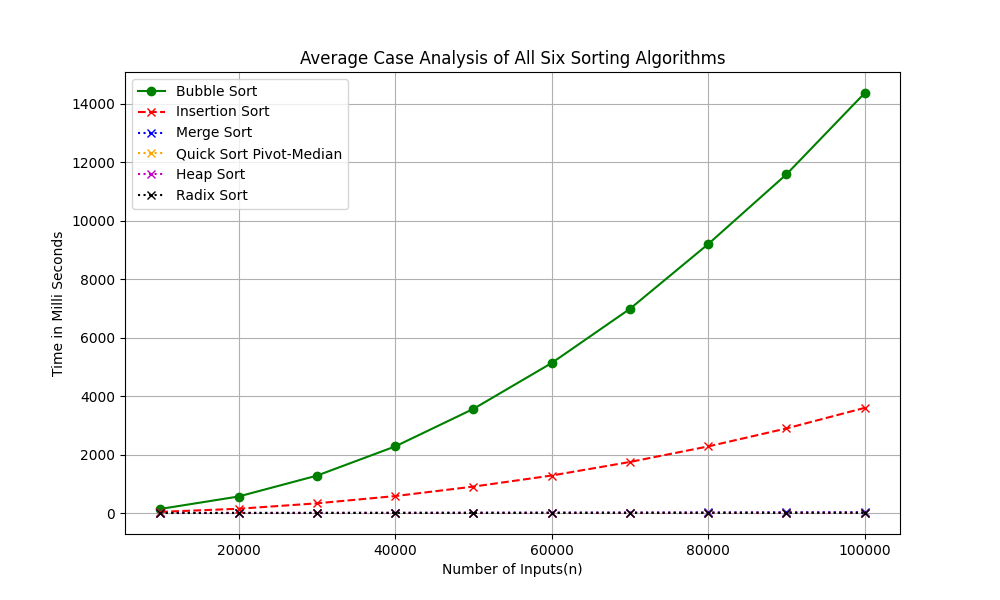
\includegraphics[width=1.1\textwidth]{./Averageofall.png}
	\caption{Average case running time of all the sorting algorithms}
	\label{fig:Average of all}
\end{figure}

\begin{figure}[H]
	\centering
	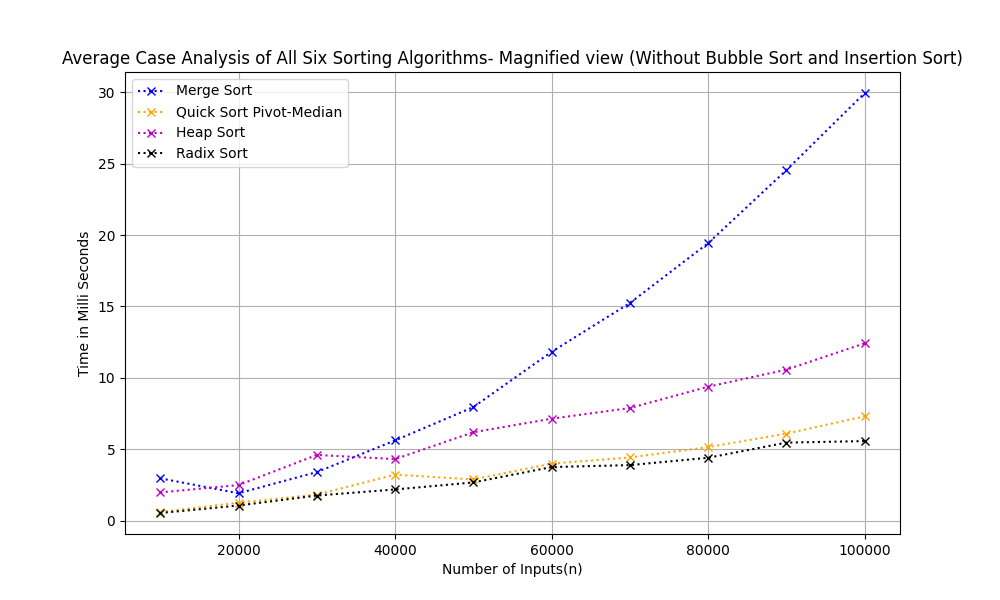
\includegraphics[width=1.1\textwidth]{./Averageofallmagnified.png}
	\caption{Average case running time of all the sorting algorithms(Magnified view: Without Bubble Sort and Insertion Sort)}
	\label{fig:Average of all Magnified}
\end{figure}

\subsection{Conclusion}
Based on the practical analysis and graphical evaluations, Radix Sort demonstrates strong performance across the best, average, and worst-case scenarios. Theoretically, the time complexity of Radix Sort is \(O(n \cdot d)\), where \(n\) represents the number of elements and \(d\) represents the number of digits in the largest number. However, if \(d\) is very, very large, the performance of Radix Sort will decrease. In my practical analysis, where \(d = 100,000\) (number of digits in the largest number), Radix Sort still performs well according to the practical analysis.
On the other hand, Quicksort with the median pivot also performs very well across the best, average, and worst-case scenarios, irrespective of the number of digits in the largest number. Therefore, when \(d\) is extremely large, Quicksort with the median pivot may be the better option.

\section{Analysis of Number of Comparisons}
Based on the following analysis, the number of comparisons for all algorithms, except Radix Sort, is correlated with execution time. This correlation indicates that as the number of comparisons increases, the execution time also tends to increase. Radix Sort does not rely on comparisons but processes individual digits instead. Comparison analysis has been conducted for all three types of inputs.
\newline
\subsection{Sorted Array in Increasing Order}
The graph clearly shows that the number of comparisons increases with input size for all sorting algorithms. Therefore, the number of comparisons is correlated with execution time.
\begin{figure}[H]
	\centering
	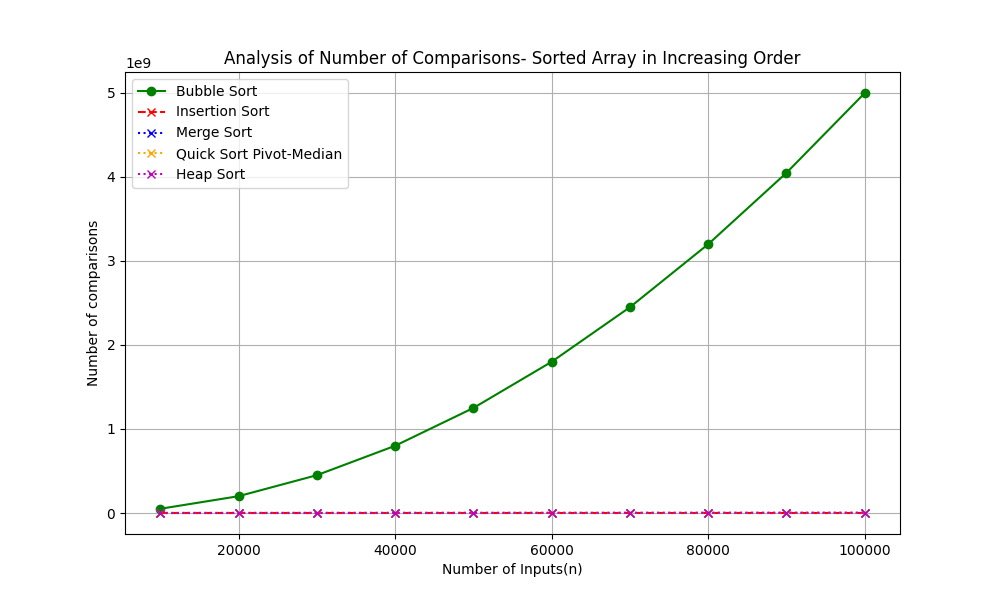
\includegraphics[width=.9\textwidth]{./Comparison_Sorted.png}
	\caption{Analysis of Number of Comparisons for  Sorted Array in Increasing Order}
	\label{fig:Comparisonsorting}
\end{figure}

\begin{figure}[H]
	\centering
	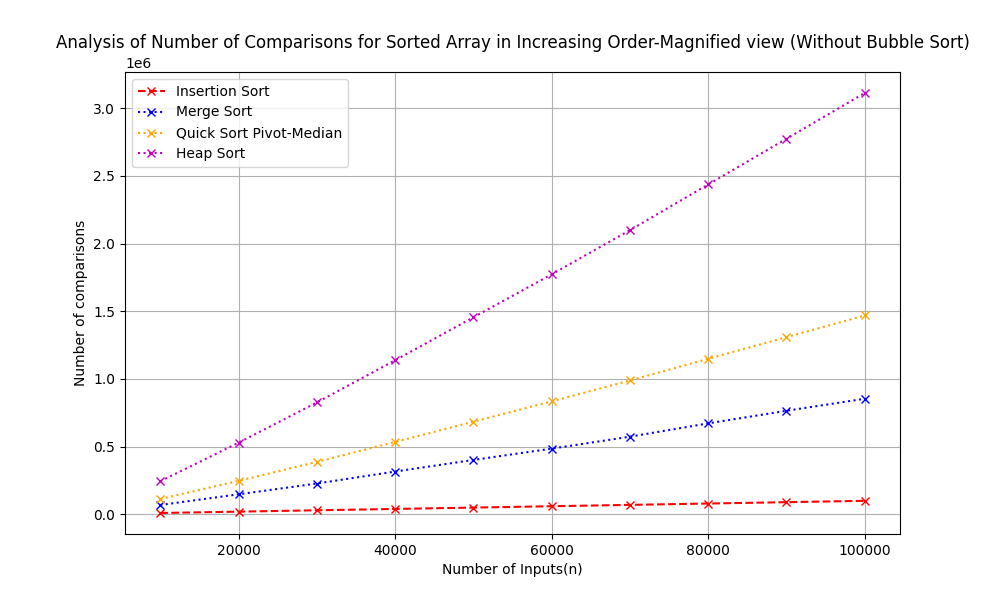
\includegraphics[width=.9\textwidth]{./Comparison_Sorted_Magnified.png}
	\caption{Analysis of Number of Comparisons for  Sorted Array in Increasing Order (Magnified view: Without Bubble Sort)}
	\label{fig:Comparisonsortingmagnified}
\end{figure}
\subsection{Sorted Array in Decreasing  Order}
The graph clearly shows that the number of comparisons increases with input size for all sorting algorithms. Therefore, the number of comparisons is correlated with execution time.
\begin{figure}[H]
	\centering
	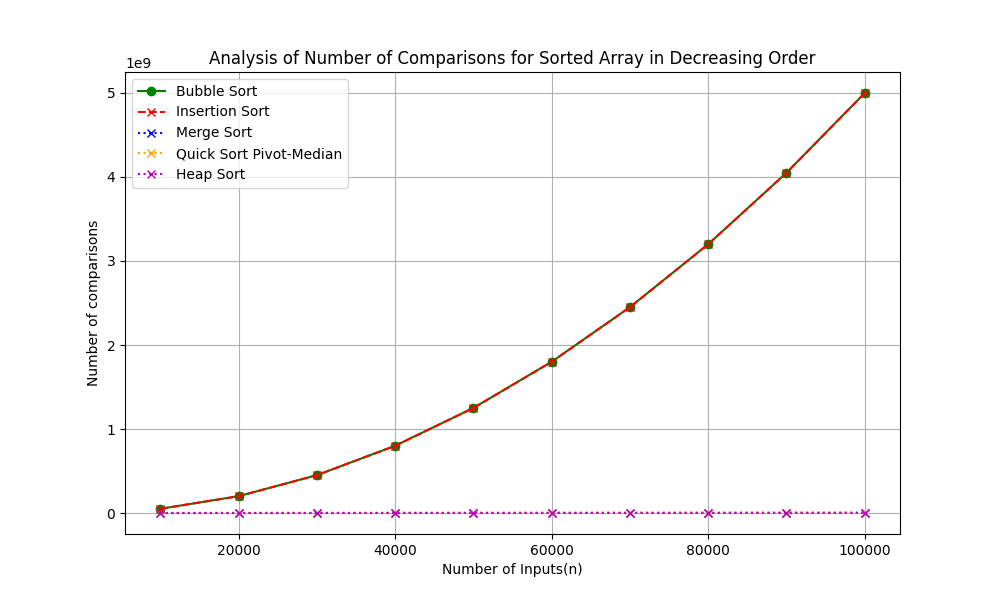
\includegraphics[width=.9\textwidth]{./Comparison_Decreasing.png}
	\caption{Analysis of Number of Comparisons for  Sorted Array in Decreasing Order}
	\label{fig:ComparisonDecreasing}
\end{figure}

\begin{figure}[H]
	\centering
	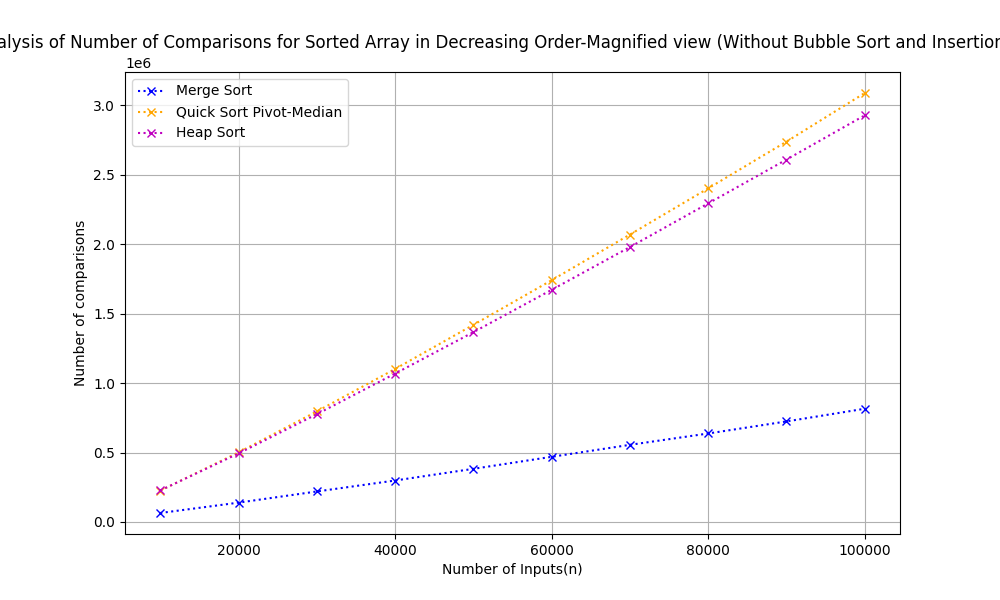
\includegraphics[width=.9\textwidth]{./Comparison_Decreasing_Magnified.png}
	\caption{Analysis of Number of Comparisons for  Sorted Array in Decreasing Order (Magnified view: Without Bubble Sort and Insertion Sort)}
	\label{fig:ComparisonsortingDecreasing}
\end{figure}

\subsection{Random Array}
The graph clearly shows that the number of comparisons increases with input size for all sorting algorithms. Therefore, the number of comparisons is correlated with execution time.
\begin{figure}[H]
	\centering
	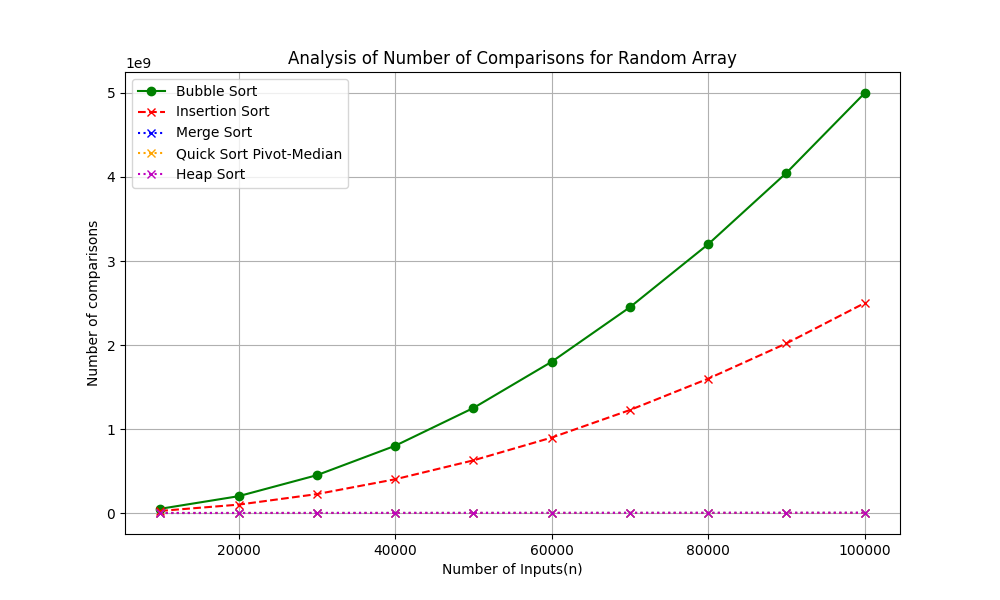
\includegraphics[width=.9\textwidth]{./Comparison_Random.png}
	\caption{Analysis of Number of Comparisons for Random Array}
	\label{fig:ComparisonRandom}
\end{figure}

\begin{figure}[H]
	\centering
	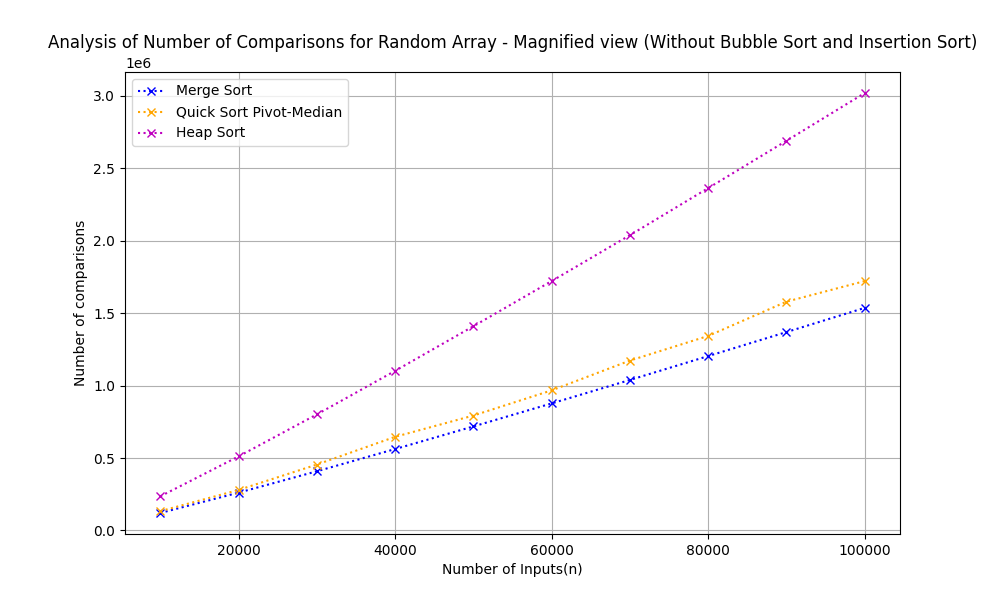
\includegraphics[width=.9\textwidth]{./Comparison_Random_Magnified.png}
	\caption{Analysis of Number of Comparisons for  Random Array (Magnified view: Without Bubble Sort and Insertion Sort)}
	\label{fig:ComparisonsortingRandom}
\end{figure}

\end{document}
